% 	/!\ Compile with LuaLaTeX
%	!TEX encoding = UTF-8 Unicode

\documentclass{Classe/Dissertate}

%	Fonts
%	/!\ Have to be installed from `font' directory before first compiling
%%%%%%%%%
% Fonts %
%%%%%%%%%

\usepackage{fontspec}

\newfontfamily\ROBL{Roboto Light}
\newfontfamily\bodyfontit[]{Roboto Thin Italic}
\newfontfamily\thinfont[]{Roboto Thin}
\newfontfamily\ROBC{Roboto Condensed}
\newfontfamily\ROBCB{Roboto Condensed Bold}
\newfontfamily\ROBCL{Roboto Condensed Light}

\newcommand*{\RobCB}{\fontfamily{phv}\selectfont}

%\defaultfontfeatures{Mapping=tex-text}
%\setmainfont[Mapping=tex-text, Color=textcolor]{Roboto Light}


%	All necessary `\usepackage' 
%\usepackage[dvipsnames]{xcolor}
\usepackage{easymat}
\usepackage{mathrsfs}
\usepackage{verbatim}
\usepackage{amsmath}
\usepackage{amssymb}
\usepackage{amsfonts}
\usepackage{mathrsfs}
\usepackage{graphicx}
\usepackage{tikz}
\usetikzlibrary{shapes.misc, positioning}
\usetikzlibrary{arrows}
\usepackage{placeins}
\usepackage{float}
\usepackage{nicefrac}
\usepackage{array}
\usepackage{stmaryrd}
\usepackage{braket}
%\usepackage[natbibapa]{apacite}
\usepackage{enumitem}
\usepackage{caption}
\usepackage{subfig}
%\usepackage{multirow}
\usepackage{array}
\usepackage{blkarray}
\usepackage{ctable}
\usepackage{arydshln}
\usepackage{bbm}
%\usepackage{graphicx}
\usepackage{pifont}
\usepackage{algorithm}
\usepackage{algorithmic}
\usepackage{hyperref}
\usepackage{bm}
\usepackage{wrapfig}
\usepackage{lscape}
\usepackage{rotating}
\usepackage{epstopdf}


%\usepackage{rotating}
%\usepackage{tabularx}
%\usepackage[labelfont=bf]{caption} % optional
%
%\usepackage{ragged2e}
%\usepackage{lipsum}%
%

%\usepackage{subcaption}
%\usepackage[table]{xcolor}
%\usepackage{multirow}

\setlength\dashlinedash{0.2pt}
\setlength\dashlinegap{1.5pt}
\setlength\arrayrulewidth{0.3pt}

% Relative folder organisation
\usepackage{import}

% Chapter-wise bibliography
\usepackage[round]{natbib}
\usepackage{bibentry}
%\usepackage{hanging}
\nobibliography*

\newcommand\hangbibentry[1]{%
    \smallskip\par\hangpara{1em}{1}\bibentry{#1}\smallskip\par %{indent}{afterline}
}
%\usepackage{chapterbib}

\usepackage{adjustbox}


%	Colors to be used for chapters 
% Chapter colors

\xdefinecolor{chapter0}{named}{black}
\xdefinecolor{chapter1}{named}{CadetBlue}
\xdefinecolor{chapter2}{named}{Salmon}
\xdefinecolor{chapter3}{named}{Apricot}
\xdefinecolor{chapter4}{named}{Thistle}
\xdefinecolor{chapter5}{named}{black}


%	Shorthands for math symbols
\renewcommand{\yen}[1]{\textcolor{blue}{#1}}

\newcolumntype{M}[1]{>{\centering\arraybackslash}m{#1}}
\newcolumntype{R}[1]{>{\raggedright\arraybackslash}m{#1}}
\newcolumntype{C}[1]{>{\centering\arraybackslash}m{#1}}

\newcommand{\tr}[1]{\textrm{tr}\left(#1\right)}

\newcommand{\bbR}{\mathbb{R}}
\newcommand{\calC}{\mathcal{C}}
\newcommand{\calF}{\mathcal{F}}
\newcommand{\calG}{\mathcal{G}}
\newcommand{\calL}{\mathcal{L}}
\newcommand{\calM}{\mathcal{M}}
\newcommand{\calN}{\mathcal{N}}
\newcommand{\calH}{\mathcal{H}}
\newcommand{\calO}{\mathcal{O}}

\newcommand{\Loss}{\text{Loss}}
\newcommand{\ot}{\leftarrow}
\newcommand{\TP}{\text{TP}}
\newcommand{\FP}{\text{FP}}
\newcommand{\TN}{\text{TN}}
\newcommand{\FN}{\text{FN}}

\newcommand{\e}{\mathrm{e}}
\newcommand{\OT}{\mathrm{OT}}
\newcommand{\bz}{\textbf{z}}
\newcommand{\bx}{\textbf{x}}
\newcommand{\by}{\textbf{y}}
\newcommand{\calZ}{\mathcal{Z}}
\newcommand{\lb}{\llbracket}
\newcommand{\rb}{\rrbracket}
\newcommand{\II}{\textbf{I}}

\newcommand{\calS}{\mathcal{S}}
\newcommand{\calX}{\mathcal{X}}
\newcommand{\calY}{\mathcal{Y}}
\newcommand{\calP}{\mathcal{P}}




\DeclareMathOperator{\dis}{dis}
\DeclareMathOperator{\dist}{dist}
\DeclareMathOperator{\dom}{dom}
\DeclareMathOperator{\expit}{expit}
\DeclareMathOperator{\calW}{\mathcal{W}}
\DeclareMathOperator{\Prox}{Prox}
\DeclareMathOperator{\sign}{sign}
\DeclareMathOperator{\var}{var}
\newcommand*{\Comb}[2]{{}^{#1}C_{#2}}%

\DeclareMathOperator{\Ind}{\textbf{1}}
\DeclareMathOperator{\GW}{\calG\calW}
\DeclareMathOperator{\diag}{diag}
\DeclareMathOperator{\card}{card}
\DeclareMathOperator{\Perm}{Perm}
\DeclareMathOperator{\Tr}{Tr}
%\DeclareMathOperator{\e}{e}
\renewcommand{\algorithmicrequire}{\textbf{Input:}}
\renewcommand{\algorithmicensure}{\textbf{Output:}}
\newcommand{\parameter}{\textbf{Parameter:}}



\DeclareMathOperator*{\argmax}{arg\,max}
\DeclareMathOperator*{\argmin}{arg\,min}

\newcommand{\specialcell}[2][c]{%
  \begin{tabular}[#1]{@{}l@{}}#2\end{tabular}}
 	
\newcommand{\indep}{\mkern2mu \rotatebox[origin=c]{90}{$\models$}\mkern2mu}
\newcommand{\defeq}{\mathrel{\vcenter{\baselineskip0.5ex \lineskiplimit0pt
                     \hbox{\scriptsize.}\hbox{\scriptsize.}}}%
                     =}
\newcommand{\eqdef}{=\mathrel{\vcenter{\baselineskip0.5ex \lineskiplimit0pt
                     \hbox{\scriptsize.}\hbox{\scriptsize.}}}
                     }
                     
\newcommand*\circled[1]{\tikz[baseline=(char.base)]{
            \node[shape=circle,draw,minimum size=12pt,draw=white,fill=#1] (char) {};}}
            
\newcommand*\circledout[1]{\tikz[baseline=(char.base)]{
            \node[shape=circle,draw,minimum size=12pt,draw= #1,fill=white] (char) {};}}

\newcommand{\niton}{\not\owns}

%	Theorem enviromnents (theorem, proposition, lemma, etc)
\usepackage{amsthm}

\newtheorem{theorem}{Theorem}[chapter]
\newtheorem{definition}{Definition}[chapter]
\newtheorem{corollary}{Corollary}[theorem]
%\newtheorem{proof}{Proof}[theorem]
\newtheorem{proposition}{Proposition}[chapter]


\newtheorem*{lemma*}{Lemma}
\newtheorem{lemma}{Lemma}[chapter]

\theoremstyle{remark}
\newtheorem{ex}{Example}[chapter]
\newenvironment{example}
  {\vspace{\baselineskip}\hrule\nopagebreak\begin{ex}}
  {\end{ex}\nopagebreak\hrule\vspace{\baselineskip}}


%	TOC per chapter
\renewcommand{\cftsecfont}{\ROBC\color{\BoxColor}}
\renewcommand{\cftsecpagefont}{\ROBC} 
\renewcommand{\cftsubsecfont}{\ROBCL}
\renewcommand{\cftsubsecpagefont}{\ROBCL} 
\renewcommand{\cftsubsubsecfont}{\ROBCL}
\renewcommand{\cftsubsubsecpagefont}{\ROBCL} 
\renewcommand{\cftsubsubsecpagefont}{\ROBCL} 
\renewcommand{\cftsecleader}{\tiny \color{\BoxColor} \cftdotfill{\cftdotsep}}
\renewcommand{\cftsubsecleader}{\hfill}
\renewcommand{\cftsubsubsecleader}{\hfill}

\newcommand{\antoine}[1]{\textcolor{orange}{~#1~}}
\renewcommand{\yen}[1]{\textcolor{blue}{~#1~}}


\makeatletter
  \def\vhrulefill#1{\leavevmode\leaders\hrule\@height#1\hfill \kern\z@}
\makeatother

\newcommand\LocalTOC{%
\vspace{-1cm}
\textcolor{\BoxColor}{\vhrulefill{1pt}}
\vspace{1cm}

\begingroup
\let\clearpage\relax
\vspace{-4.9cm}
\localtableofcontents*
\endgroup

\noindent\textcolor{\BoxColor}{\vhrulefill{1pt}}

\vspace{0.5cm}
  }

%	Color index on the side
%	Use '\ChangeColor' to change color
\usepackage{background}
\usetikzlibrary{positioning,calc}
\usepackage{ifthen}
%\usepackage{titleps}

%\renewcommand{\chaptermark}[1]{\markboth{\thechapter. {\slshape{##1}}}{}}

\def\tikzmark#1{\tikz[remember picture, overlay]\coordinate(#1);}

\newcommand\OddChapter{%
\ifthenelse{\isodd{\thepage}}
{\newpage 
\Framefalse
\thispagestyle{empty}
~
\newpage
\Frametrue
}
{
}
}

% background common settings
\SetBgScale{1}
\SetBgAngle{0}
\SetBgOpacity{1}
\SetBgContents{}

% auxiliary counter
\newcounter{chapshift}
%\addtocounter{chapshift}{-1}


\newif\ifFrame
\Frametrue

\newcommand\ChangeColor{%
\stepcounter{chapshift}
  }

% the list of colors to be used (add more if needed)
\newcommand\BoxColor{%
  \ifcase\thechapshift chapter0\or chapter1\or chapter2\or chapter3\or chapter4\else chapter5\fi}
 
  
  \newcommand\ChapterColor{%
  \colorlet{chaptergrey}{\BoxColor}}


% the main command; the mandatory argument sets the color of the vertical box
\makeatletter
\newcommand\ChapFrame{%
\AddEverypageHook{%
\ifFrame
\ifthenelse{\isodd{\thepage}}
{\SetBgContents{%
  \begin{tikzpicture}[overlay,remember picture]
  \node[fill=black!5,inner sep=2pt,rectangle,text width=0.4cm,
    text height=297mm,align=center,anchor=north east] 
  at ($ (current page.north east) + (-0cm,-0.5cm)$) 
  {};
  \node[fill=\BoxColor,inner sep=2pt,rectangle,text width=0.4cm,
    text height=7cm,align=center,anchor=north east] 
  at ($ (current page.north east) + (-0cm,-7*\thechapshift cm) + (-0cm,-1cm) + (-0cm,-0.5cm)$) 
  {\rotatebox{90}{~\parbox[c][0.3cm][t]{6cm}{%
    \raggedright\textcolor{white}{\ROBCL \variable}}}};
  \end{tikzpicture}}%
}
{\SetBgContents{%
  \begin{tikzpicture}[overlay,remember picture]
      \node[fill=black!5,inner sep=2pt,rectangle,text width=0.4cm,
    text height=\paperheight,align=center,anchor=north west] 
  at ($ (current page.north west) + (-0cm,-0.5cm)$) 
  {};
  \node[fill=\BoxColor,inner sep=2pt,rectangle,text width=0.4cm,
    text height=7cm,align=center,anchor=north west] 
  at ($ (current page.north west) + (-0cm,-7*\thechapshift cm) + (-0cm,-1cm) + (-0cm,-0.5cm)$) 
  {\rotatebox{90}{~\parbox[c][0.3cm][t]{6cm}{%
    \raggedright\textcolor{white}{\ROBCL \variable}}}};
  \end{tikzpicture}}
}
\bg@material%
\fi%
}%
}

%\def\AtBeginChapter{\g@addto@macro\@beginchapterhook}
%
%
%\def\AtEndChapter{\g@addto@macro\@endchapterhook}
%
%\ifx\@beginchapterhook\@undefined
%  \let\@beginchapterhook\@empty
%\fi
%
%\ifx\@endchapterhook\@undefined
%  \let\@endchapterhook\@empty
%\fi

\makeatother


%\AtBeginChapter
%{
%\ChangeColor%
%\ChapFrame%
%\LocalTOC%
%}
%
%\AtEndChapter
%{
%\OddChapter%
%}


%	Footer flipbook a
%	Images stored in 'animation', numbered 0,2,4, etc.
%	Use '\BeginAnimation' to start the flipbook
%	Use '\Animefalse' to stop the flipbook
\usepackage{everyshi}

\newif\ifAnime
\Animetrue

\makeatletter
\newcommand\BeginAnimation{%
  \newcounter{animation}
%  \setcounter{animation}{-1}
  \EveryShipout{\stepcounter{animation}}
  
%   \newcounter{animationO}
%  \setcounter{animationO}{-1}
%   \EveryShipout{\stepcounter{animationO}}
  
  
\AddEverypageHook{%
\ifAnime
\ifthenelse{\isodd{\thepage}}
{\SetBgContents{%
  \begin{tikzpicture}[overlay,remember picture]
  \node[inner sep=0pt,align=center,anchor=south east] at ($ (current page.south east) + (-0.5cm,-0.2cm)$)
    {\includegraphics[width=.15\textwidth]{animation/\theanimation}};
  \end{tikzpicture}}%
}
{%
%\SetBgContents{%
%  \begin{tikzpicture}[overlay,remember picture]
%  \node[inner sep=0pt,align=center,anchor=south west] at ($ (current page.south west) + (0.5cm,-0.2cm)$)
%    {\includegraphics[width=.15\textwidth]{animation/\theanimationO}};
%  \end{tikzpicture}}%
}%
\bg@material%
\fi%
}%  
}
\makeatother 
  



\bibliographystyle{abbrvnat}
\usepackage{pdfpages}


\begin{document}
 \setcounter{page}{1}
 \pagenumbering{roman}
 
%	Frontpage, to be compiled beforehand 
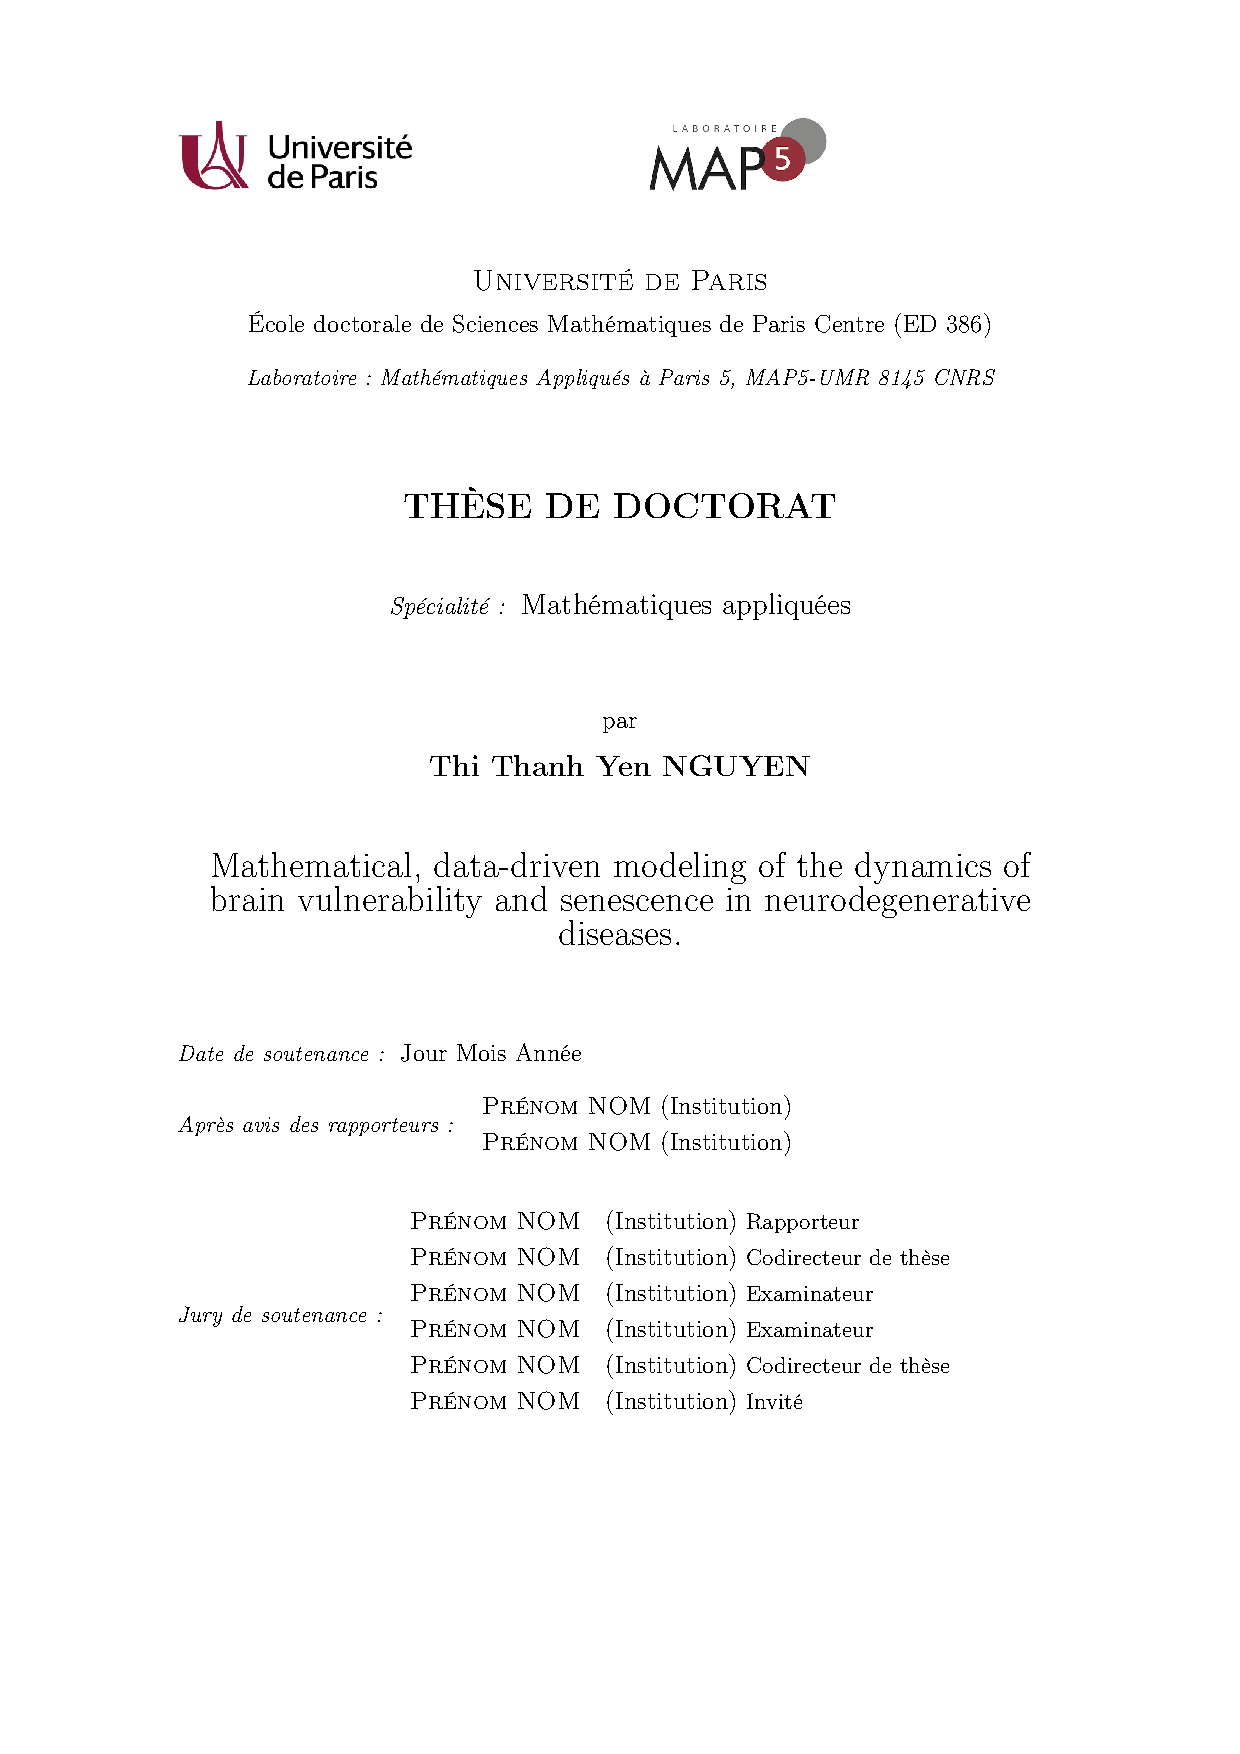
\includepdf{Frontpage/frontpage.pdf}
%
% Thesis information (title, director, etc)
%!TEX root = ../dissertation.tex
% Some details about the dissertation.
\title{Title of the dissertation}
\author{John Doe}

%If you have one advisor
\advisor{John (II) Doe}

\committeeInternalOne{}
\committeeInternalTwo{}

%If you are coadvised
\coadvisorOne{John (II) Doe}
\coadvisorTwo{Jane Doe}
\committeeInternal{}

% Everyone has an External committee member
\committeeExternal{}

% ... about the degree.
\degree{Doctor of Philosophy}
\field{Mathematics}
\degreeyear{2050}
\degreeterm{Fall}
\degreemonth{October}
\department{Mathematics}

% ... about the candidate's previous degrees.
\pdOneName{}
\pdOneSchool{}
\pdOneYear{}

\pdTwoName{}
\pdTwoSchool{}
\pdTwoYear{}

%\frontmatter

    \lab
    %\abstractpage
    %\dedicationpage
    %
    
    
        
%!TEX root = ../dissertation.tex
% the abstract
\noindent {\large{\ROBCB Abstract}}\\

Optimal transport theory has found many application in diverse fields in machine learning thank to 
providing a powerful tool for comparing probability distributions, one of a crucial issue
in machine learning.  In this thesis, we leverage the optimal transport theory and statistics to deal with 
the problems in biology and actuary. We develop new methodology based on evaluating OT distance
between empirical distributions attached on real datasets and turn it into a loss function for optimisation
using a mini-batch gradient descent and Sinkhorn algorithm.  


%This thesis presents the applications of the Optimal Transport theory and  
%statistics in two domains: biology and actuary. We learn the Sinkhorn 
%divergence, a classe of discrepancies between objects, based on regularized
%OT distance to discover the patterns of datasets. The Sinkhorn divergence is 
%considered as the loss function which we want to minimize using a mini-batch
%gradient descent and Sinkhorn algorithm.  \\
In the first part of this thesis, we  present  several  algorithms  designed   to
learn  a  pattern  of correspondence between two data sets in  situations where
it is desirable to match elements that  exhibit a relationship belonging to  a known parametric
model.  The algorithms unfold  in two stages.  First, an  optimal transport plan
and an optimal  affine transformation are learned. Second,  the OT matrix is  exploited to
derive either several co-clusters or several sets of matched elements.\\
In the second part,  we develop a new methodology to anticipate which cities will request
a declaration  of natural disaster  for a drought event,  a key step  of the
national compensation  scheme. We build an  inertial proximal algorithm for  nonconvex optimization.  
The optimisation  problem  is  designed  so  as to  yield  a  sparse  vector  of
predictions because  it is known  that relatively  few cities will  make the
request.

  
  \textbf{Keywords.} Optimal transport; Sinkhorn algorithm; Sinkhorn divergence;
  proximal algorithm; matching; Huntington's disease; omics data; natural disasters.
  
       
  
~\newpage
\vspace{0.1cm}
%!TEX root = ../dissertation.tex
% the abstract
\selectlanguage{french}

\noindent{\large{\ROBCB Résumé}}\\

Cette thèse présente les applications de la théorie du Transport Optimal et des statistiques dans deux domaines : la biologie et l'actuariat. Nous apprenons la divergence de Sinkhorn, une classe de divergences entre objets, basée sur la distance OT régularisée pour découvrir les modèles des ensembles de données. La divergence de Sinkhorn est considérée comme la fonction de perte que nous voulons minimiser en utilisant une descente de gradient en mini-batch et l'algorithme de Sinkhorn.\\
Dans la première partie de cette thèse, nous présentons plusieurs algorithmes conçus pour apprendre un motif de correspondance entre deux ensembles de données dans des situations où il est souhaitable de faire correspondre des éléments qui présentent une relation appartenant à un modèle paramétrique connu. Les algorithmes se déroulent en deux étapes. Premièrement, un plan de transport optimal et une transformation affine optimale sont appris. Ensuite, la matrice OT est exploitée pour dériver soit plusieurs co-clusters, soit plusieurs ensembles d'éléments appariés.\\
Dans la deuxième partie, nous développons une nouvelle méthodologie pour anticiper les villes qui demanderont une déclaration de catastrophe naturelle pour un événement de sécheresse, une étape clé du système d'indemnisation national. Nous construisons un algorithme proximal inertiel pour l'optimisation non convexe. Le problème d'optimisation est conçu de manière à produire un vecteur clairsemé de prédictions car on sait que relativement peu de villes feront la demande.


\noindent {\ROBCB Mots-Clefs :} Algorithme de Sinkhorn; contraste de Sinkhorn; co-clustering spectral; g\'enomique; maladie de Huntington; matching; transport optimal.

\selectlanguage{english}




~\newpage
 %\acknowledgments
%!TEX root = ../dissertation.tex
% the acknowledgments section
%\selectlanguage{french}

\noindent{\large{\ROBCB Remerciements}}\\

Merci à Warith, qui m'a enseigné d'utiliser le Python et partager les idées.

Merci à toi Olivier, qui m'a fait confiance il y a maintenant de cinq ans. Ton soutien 
permanent, qu'il soit scientifique ou amical.

Pour finir, j'aimerais te remercier, Antoine, très sincèrement. 

Un très grand merci à Anne et Fabienne pour leur soutien indéfectible, à Marie- Hélène, ...,
 et l'ensemble des équipes administratives et techniques pour leur aide si précieuse durant ces années passées au MAP5. Une salutation générale pour tous ceux, permanents ou passagers, que j'ai pu croiser et côtoyer, et qui contribuent à cette ambiance si particulière et chaleureuse de MAP5 que j'ai envie de nommer l'esprit terrasse de 7ème. 

Merci aux tous fameux éphémères de MAP5. 

Merci à Safa et Ousmane de partager les bonnes moments et de compagne longtemps.

Merci à Florian, Charlie, Antoine Monod. 

En fin, 


%\selectlanguage{english}

~\newpage
%\Notations and Definitions
%!TEX root = ../dissertation.tex
% the notations and definitions sections.

\noindent{\Large{\ROBCB Notations and definitions}}\\

\noindent{\large{\ROBCB Definitions}}\\

\noindent{\large{\ROBCB Notations }}\\
\begin{itemize}
\item $\llbracket M \rrbracket:$ set of integers $\{1, \ldots, M\}$.
\item $\Omega_M:$ probability simplex with $M$ bins, namely the set of probability vectors in $\bbR_+$.
\item $\mathbf{1}_M:$ vector of size $M$ with all entries equal to 1.
\item $\textbf{0}_d:$ vector of size $d$ with all entries equal to 0.
\item $c(x,y):$ cost function, with associated pairwise cost matrix $(C(\bx, \by))_{m,n} =c(x_m, y_n)$ evaluated on $\bx$ and $\by$.
\item $(a, b):$ histograms in the simplices $\Omega_M \times \Omega_N$.
\item$(\alpha, \beta)$ probability measures, defined on spaces $(\calX, \calY)$
\item $\Pi(a, b):$ set of couplings between vectors $a, b$.
\item $\Pi(\alpha, \beta):$ set of couplings between measures $\alpha, \beta$.
\item $(\mu_{\bx}^{a} := \sum_{m\in \llbracket M \rrbracket} a_m \delta_{x_m}  , \nu_{\by}^{b} := \sum_{n\in \llbracket N \rrbracket} b_n \delta_{y_n}):$ the weighted empirical measure attached to $\bx := \{x_1,\ldots, x_M \}$ and $\by := \{y_1, \ldots, y_N\}$, respectively.
\item For $\rho \in \bbR^{M}$,  $\diag(\rho)$ is the $M\times M$ matrix with diagonal $\rho$ and zero otherwise.
\item $OT_{c} (\alpha, \beta)$: value of optimization problem associated to the optimal transport with cost function $c$.
\item $\langle \cdot, \cdot \rangle_{F}:$  for the usual Euclidean dot-product between vectors; for two matrices of the same size $A$ and $B$, $\langle A, B\rangle_{F} := \Tr{A^{\top} B}$ is the Frobenius dot-product.
\item $K := \mathrm{e}^{-C/\gamma}$   Gibbs kernel associated to the cost matrix $C$.
\item $ a \otimes b := a b^\top \in \bbR^{M\times N} $.
\item $ a \odot b := (a_m b_m) \in \bbR^M$ for $(a, b) \in (\bbR^M)^2$.
\item $\mathbf{f}  \oplus  \mathbf{g} := \mathbf{f}  \mathbf{1}_M^\top + \mathbf{1}_N \mathbf{g}^\top \in \bbR^{M \times N}$ for two vectors $\mathbf{f} \in \bbR^M$, $\mathbf{g} \in \bbR ^{N}$
\end{itemize}
\noindent{\large{\ROBCB Abbreviations }}\\

\noindent{\large{\ROBCB Conflicts in notation between chapters }}\\
We have tried to use coherent and non-conflicting notation for the mathematical objects defined in this thesis. However, for the sake of consistency with the conventions of the field, we made the choice to keep conventional notations for known quantities. ...\\
\yen{add more detail, where there are conflict}\\
Theses notational conflicts have been kept to ease the understanding of the manuscript. They occur between different chapters but not inside each chapter. We stress that the potential uncertainty is removed when the context is taken into consideration.












    \tableofcontents
     
    \clearpage
    
    \OddChapter%
    
	\setcounter{page}{1}
    \pagenumbering{arabic}
    \restoregeometry
    
\renewcommand{\contentsname}{}
\setcounter{tocdepth}{3}
\addtocounter{chapter}{0}


\ChangeColor%
\chapter{Introduction}
%\ChapFrame%
\LocalTOC%
\subimport{Chapters/Ch_Resume/}{ch_resume.tex}
\OddChapter%
\clearpage


\ChangeColor%
\chapter{Elements of transport optimal}
%\ChapFrame%
\LocalTOC%
\subimport{Chapters/Ch0/}{ch0.tex}
\OddChapter%
\clearpage



\ChangeColor%
\chapter{Optimal transport-based machine learning to match specific patterns: application to the detection of molecular regulation patterns in omics data}
\ChapFrame%
\LocalTOC%
\subimport{Chapters/Ch1/}{ch1.tex}
\OddChapter%
\clearpage
%

\ChangeColor%
\chapter{Making sparse predictions, and anticipating the requests of declaration
  of natural  disasters for a drought  event in France}
\ChapFrame%
\LocalTOC%
\subimport{Chapters/Ch2/}{ch2.tex}
\OddChapter%
\clearpage

\ChangeColor%
\chapter{Conclusion and discussion}
\ChapFrame%
\LocalTOC%
\subimport{Chapters/Ch3/}{ch3.tex}
\OddChapter%
\clearpage

%\ChangeColor%
%\chapter{Sparse prediction}
%\ChapFrame%
%\LocalTOC%
%\subimport{Chapters/Ch3/}{ch3.tex}
%\OddChapter%
%\clearpage


%
%\ChangeColor%
%\chapter{En Bref}
%\Framefalse
%\ChapFrame%
%\subimport{Chapters/Ch_Resume/}{ch_resume.tex}
%\OddChapter
%\clearpage
%
%\ChangeColor
%\chapter*{Published Articles and Preprints}
%\Framefalse
%\Animefalse
%\ChapterColor

%\begin{list}{}{%
\setlength{\topsep}{0pt}%
\setlength{\leftmargin}{1em}%
\setlength{\listparindent}{-1em}%
\setlength{\itemindent}{-1em}%
\setlength{\parsep}{\parskip}%
}%
\item[]
\bibentry{Me2050}

\vspace{0.5\baselineskip}

\item[]
\bibentry{Me2051}
\end{list}

\bibliography{References/main}
%\bibliography{References/sparse_regression}
\newpage
\pagestyle{empty}
%\OddChapter
~ 
\newpage



\end{document}
